\begin{figure}[!ht]
\centering
\resizebox{\columnwidth}{!}{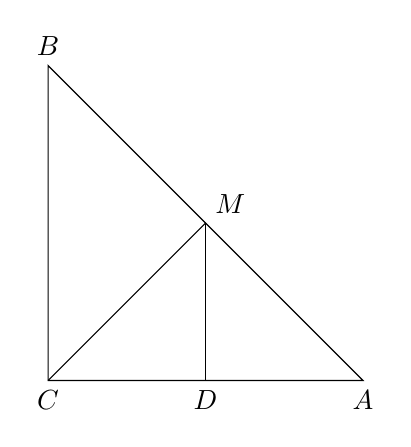
\begin{tikzpicture}
\coordinate (B) at (0,4);
\coordinate (A) at (4,0);
\coordinate (C) at (0,0);
\coordinate (D) at (2,0);
\coordinate (M) at (2,2);
\draw (A)node[below]{$A$}--(B)node[above]{$B$}--(C)node[below]{$C$}--cycle;
\draw(M)node[above right]{$M$}--(D)node[below]{$D$};
\draw(M)--(D);
\draw(M)--(C);
\tkzMarkRightAngle(B,C,A)
\tkzMarkRightAngle(A,D,M)
\tkzMarkRightAngle(C,D,M)
\end{tikzpicture}
}
\caption{Triangle ABC and DBC}
\label{eq:solutions/1/27/myfig}
\end{figure}
In $\triangle{ABC}$, $\vec{M}$ is midpoint of hypotenuse AB, thus 
\begin{align}
&\vec{M} = \frac{\vec{A}+\vec{B}}{2}\label{eq:solutions/1/27/eq1} \\
&2\vec{M} = \brak{\vec{A+B}}\\
&\brak{\vec{A-M}} = \brak{\vec{M-B}}\\
&\norm{\vec{A}-\vec{M}}=\norm{\vec{M}-\vec{B}}\label{eq:solutions/1/27/eq4} \\
&\vec{M} = \frac{\vec{C}+\vec{D}}{2}\label{eq:solutions/1/27/eq2} \\
&2\vec{M} = \brak{\vec{C+D}}\\
&\brak{\vec{C-M}} = \brak{\vec{M-D}}\\
&\norm{\vec{C}-\vec{M}}=\norm{\vec{M}-\vec{D}}\label{eq:solutions/1/27/eq5} \\
&\vec{M} = \frac{\vec{A}+\vec{B}}{2} = \frac{\vec{C}+\vec{D}}{2}\label{eq:solutions/1/27/eq3} \\
&\vec{A - C} = \vec{A - M} + \vec{M - C} \\
&\vec{A - C} = \vec{M - B} + \vec{D - M} \\
&(\vec{A - C}) = k(\vec{D - B})\label{eq:solutions/1/27/eq6} \quad\text{[k value is 1]}
\end{align} 
Now from equation \eqref{eq:solutions/1/27/eq6} we can say that 
\begin{align}
&AC \parallel DB\label{eq:solutions/1/27/eq8} \\
&\norm{\vec{A - C}} = \norm{\vec{D - B}}\label{eq:solutions/1/27/eq7} 
\end{align}
Now it is given that AC $\perp$ BC, using this we can prove that DB $\perp$ BC. 
\begin{align}
&(\vec A -\vec C)^T(\vec{B}-\vec{C}) = 0 \\
&(\vec A -\vec M +\vec M -\vec C)^T(\vec{B}-\vec{C}) = 0 \\
&(\vec M -\vec B +\vec D -\vec M)^T(\vec{B}-\vec{C}) = 0 \\
&(\vec D -\vec B)^T(\vec{B}-\vec{C}) = 0 \\
&\implies DB \perp BC \\
&\vec{A - B} = \vec{A - C}+\vec{C - B} \\
&\vec{A - B} = \vec{B - D}+\vec{C - B} \quad\text{[From \eqref{eq:solutions/1/27/eq7}]} \\
&\vec{A - B} = \vec{C - D} \\
&\vec{A - B} = \vec{C - M}+ \vec{M - D} \\
&\vec{A - B} = \vec{C - M}+\vec{C - M} \quad\text{[From \eqref{eq:solutions/1/27/eq5}]}
\end{align} 
\begin{align}
&\vec{A - B} = 2 (\vec{C - M}) \\
&\vec{C - M} = \frac{1}{2}(\vec{A - B}) \\
&\norm{\vec{C - M}} = \frac{1}{2}\norm{\vec{A - B}}\label{eq:solutions/1/27/eqFin1}
\end{align}
Hence from \eqref{eq:solutions/1/27/eqFin1} proved,\\CM = $\frac{1}{2}$ AB
